% !TEX root = ../main_orange.tex

We will now go though the main aspects of how different particles are reconstructed by ATLAS. This discussion will be crucial to understand the variables that are available for this experiment. 

\section{The ATLAS detector}

ATLAS is a general-purpose particle detector operating at a hadron collider. The structure of the detector is sometimes referred to as onion-like, because different layers of detectors are present when going from the collision point outwards. A detailed description of the ATLAS detector and the technologies used for particle detection goes well below the scope of this document: if you are interested please refer to Ref.~\cite{Aad:2008zzm}. What we will do here is to summarise the main principles behind particle detection.

\begin{figure}[tb] 
	\centering
	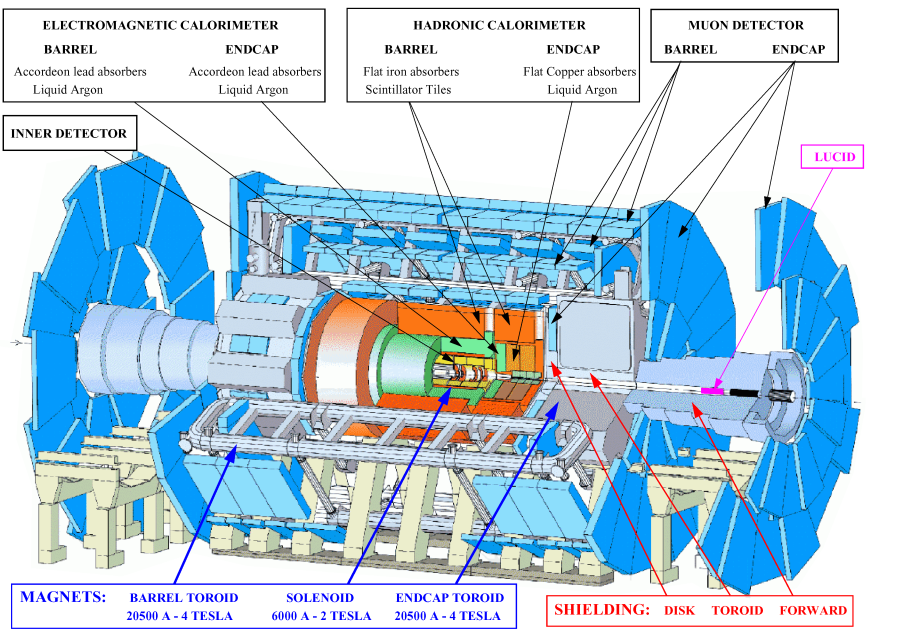
\includegraphics[width=0.7\columnwidth]{Figures/atlas.png}
	\label{fig:ATLAS}
	\caption{Overview of the ATLAS detector. Taken from Ref.~\cite{ATLAS_detector_image}}
\end{figure}

Figure~\ref{fig:ATLAS} shows the various components of ATLAS. Starting from the collision point and going outward: 

\begin{itemize}

\item \textbf{Inner Detector (ID):} Starting at about 3 cm away from the collision point, the inner detector is optimised to measure the position of charged particles. It is immersed in a magnetic field directed along the $z$ axis, such that charged particles trajectories are bent. From the curvature radius it is possible to measure the particle momentum transverse to the magnetic field. 

\begin{exercise}
Remembering that $\mathbf{F} = q \mathbf{v} \times \mathbf{B}$ is acting as centripetal force, estimate the curvature radius of a particle with unit charge and momentum $p = 10\ \GeV$ if $B = 2$~T. 
\end{exercise}

\item \textbf{Electromagnetic (EM) calorimeter:} It stops electrons and photons and measures their energy. It also participate in the energy measurement of hadrons. 
\item \textbf{Hadronic (HAD) calorimeter:} Together with the electromagnetic calorimeter, it measures the energy of neutral and charged hadrons. 
\item \textbf{Muon spectrometer (MS):} Muons and neutrinos are the only particles in the SM that are able to exit the ATLAS calorimeters. The principle of the muon spectrometer is similar to that of the inner detector: the position of muons is measured several times while they are bending in a magnetic field generated by the air-core toroids. From that, a second measurement of the muon momentum is performed, which is typically  combined with the first one taken by the ID. 
\end{itemize}

The subdetectors outlined above are used in combination to reconstruct a number of different final state ``objects''. The number of types of objects which is normally used in an analysis is actually relatively limited. The main features of each of these objects is reviewed below. 

\begin{itemize}
\item{Electrons:} they are identified by a cluster of energy in the EM calorimeter matched with a track in the ID. \textit{Shower shape variables} (that is, the shape of the cluster in the calorimeter), the track quality, and the quality of the matching between the cluster and the track (are the track momentum and cluster energy compatible?) determine the identification. 
\item{Photons:} similar to electrons for the cluster in the EM calorimeter, but with no associated track in the ID. 
\item{Muons:} a track in the MS is almost uniquely identifying a muon (no other charged particle pass through the calorimeters). Typically the MS track is matched to one in the ID. 
\item{Jets:} Quarks and gluons cannot emerge from a collision as such. They go through a process of fragmentation and hadronisation~\cite{fragment_hadronise}, resulting in a jet of collimated hadrons, whose total momentum and direction resembles that of the originating quark/gluon. Such jets are reconstructed mainly from the HAD and EM calorimeter information, but they use some information from the ID as well. 
\item{$b$-jets:} $b$-quarks have a longer lifetime than the other quarks. They travel of the order of a cm or less before decaying. The presence of such secondary vertex (that is, a vertex that does not coincide with the primary one from the pp collision in the transverse plane) can be exploited to ``tag'' the jet as originating from a $b$.
\item{$\tau$ leptons:} The lifetime of the $\tau$ is extremely short. For all practical purposes, it decays before producing any visible effect in the detector. There are two main categories of $\tau$ decays: the leptonic ones and the hadronic ones. If a $\tau$ decays to an electron and muon (through $\tau\rightarrow \ell \bar{nu}_{\ell} \nu_{\tau}$ to conserve the lepton number and flavour), it will be seen as a lepton in the detector. If instead a tau decays to hadrons, then it looks like a very narrow jet with few tracks attached, and it can be identified based on these characteristics. 
\item{Invisible particles:} If an invisible particle is produced (neutrinos, in the standard model), their presence is inferred from the measurement of the total momentum transverse to the beam. Given that the momentum in the plane transverse to the beam is zero before the proton-proton collision, it has to be zero after the collision. The negative vectorial sum of the transverse momenta of all object in the events is called the \textit{missing transverse momentum}, and is an estimate of the total transverse momentum of invisible particles.   
\end{itemize}

Figure~\ref{fig:ttbar_eventdisplay} shows a candidate event for $t\bar{t} \rightarrow \mu \nu_{\mu} + 4\ \mathrm{jets}$. See the caption for further details. 

\begin{figure}[tb] 
	\centering
	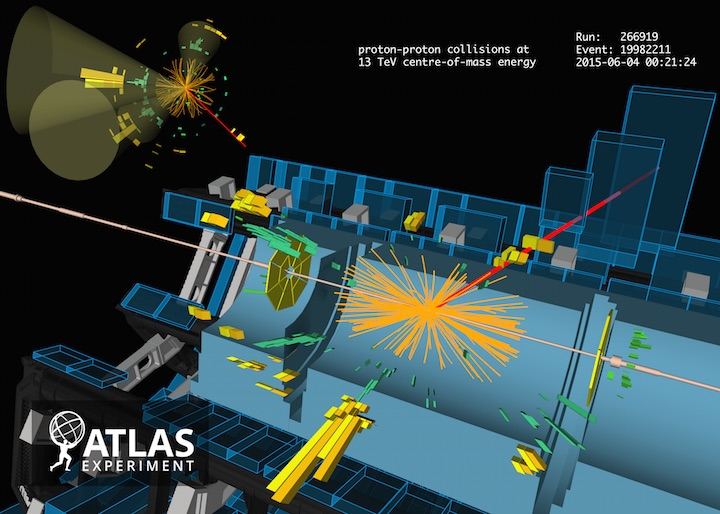
\includegraphics[width=0.7\columnwidth]{Figures/ATLAS_ttbar_candidate_13TeV_VP1_run266919_evt19982211_thumb.jpg}
	\label{fig:ttbar_eventdisplay}
	\caption{Display of a $t\bar{t}$ candidate event from proton-proton collisions recorded by ATLAS at a collision energy of 13 TeV. The red line shows the path of a muon with transverse momentum around 35 GeV through the detector. The green and yellow bars indicate energy deposits in the EM and HAD. From close-by deposits in these calorimeters, four jets are identified with transverse momenta between 25 and 80 GeV. Taken from Ref.~\cite{ATLAS_ttbar_evtdisplay}}
\end{figure}

\section{Monte Carlo and real events}

In this experiment you will deal with two types of events: simulated and real ones. The simulated ones are often referred to as Monte Carlo, or simply MC, events. MC events are the result of a computer simulation, that emulates at best the theory we have for the proton-proton collision. They simulate a specific process (like $Z$ production, or $H$ production), they save the so called truth-level information (that is, the particles that were produced in the collision and that enter the detector) and they also simulate the response of the detector (reco-level). The MC represents our theoretical prediction. 

%It is probably worth at this stage to introduce the concept of cross-section weight. Suppose that I simulate $N$ events of a process whose cross-section is $\sigma$. I know that the data I will be looking at correspond to an integrated luminosity $L$. If I want 

